\hypertarget{ux6458ux8981}{%
\section*{摘要}\addcontentsline{toc}{section}{摘要}\label{ux6458ux8981}}

本项目研究如何让视觉策略在 Adroit 灵巧手环境中完成笔的目标姿态重定向。我们首先从 25 条 human demonstrations 中恢复 5,000 个源状态，并在严格排除跨 episode 边界后得到 4,975 条合法离线 transition，以 Behavior Cloning（BC）、critic warm-up 和 offline AWAC 建立视觉控制基线。随后，RGB 黑屏、跨 episode 打乱和目标遮挡实验表明图像内容确实影响策略，但时间顺序打乱几乎不降性能，暴露出基础视觉表征对动态信息利用不足。Direct PPO、Residual SAC、安全残差、反事实分支监督与候选排序均未能稳定改善接触敏感闭环：问题并非只有动作改动过大，更在于用稀疏长时结果可靠判断微小修正的收益十分困难。最终，我们把问题从``此刻应该怎样改动作''改写为``此刻物体的隐含物理状态是什么''，提出 Temporal Visual-State Distillation：利用 544 条仿真轨迹、108,800 个时序样本，以 privileged state 和 Frozen Oracle action 作为训练监督，学习仅依赖 8-step RGB、proprioception 与历史动作的因果状态估计器，再经冻结 Oracle AWAC 输出动作。固定 E2 在独立 300-episode paired confirmation 上将 Benchmark 从 52.3\% 提升至 68.3\%，Strict 从 27.0\% 提升至 37.0\%；在一次性 200-episode frozen test 上，Benchmark 从 54.5\% 提升至 75.0\%，Strict 从 26.0\% 提升至 33.5\%。项目完全处于仿真环境，没有 sim-to-real 或真实硬件结果；长期 hold、训练 seed 方差和 frozen-test Strict 的统计不确定性仍是明确限制。

\begin{figure}
\centering
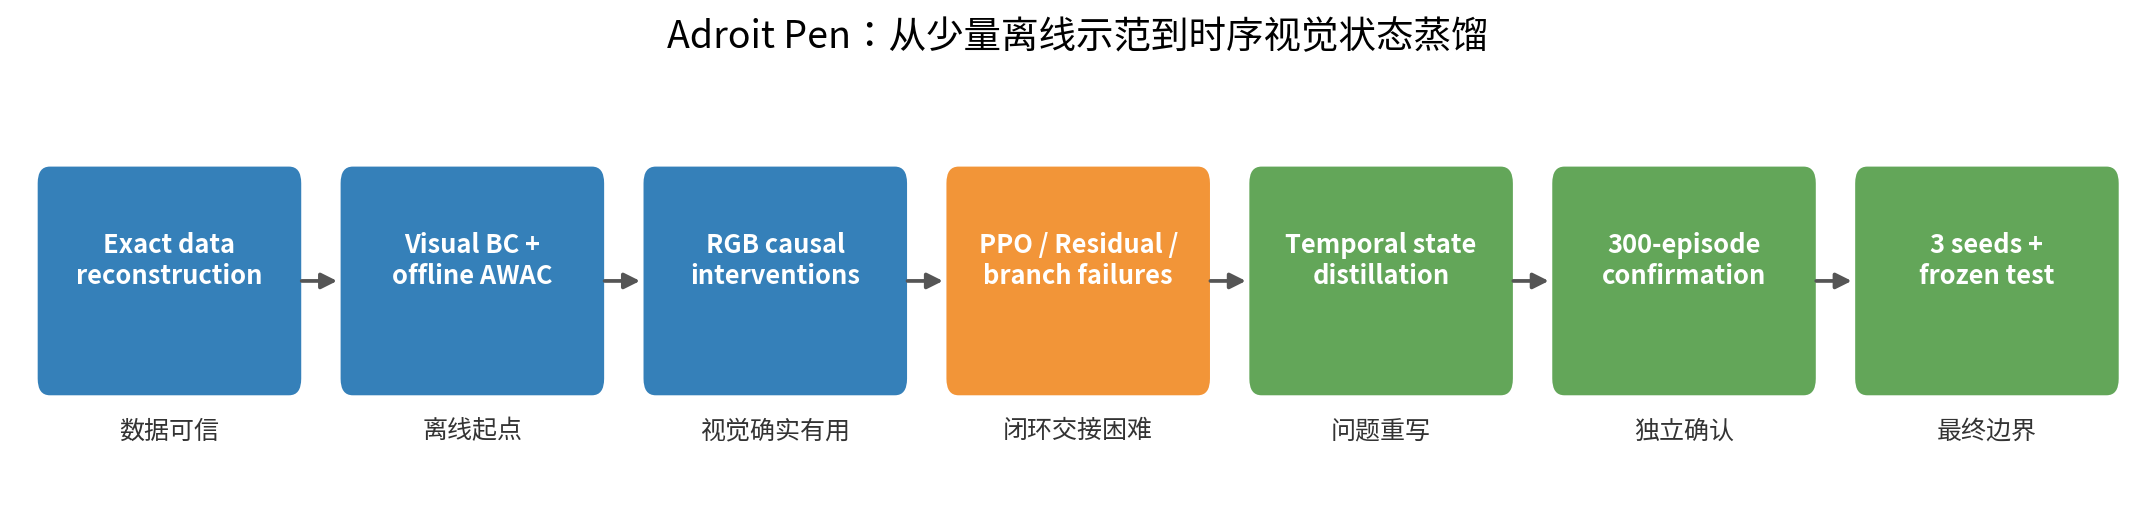
\includegraphics[width=\linewidth]{figures/01_research_route.png}
\caption{总体研究路线：从数据恢复到时序视觉状态蒸馏}
\end{figure}

\textbf{图 1｜总体研究路线。} 图中各阶段来自不同开发或评测 bank，不是同一条学习曲线。它表达的是问题求解顺序：先验证数据和视觉因果性，再利用失败实验定位 offline-to-online 交接困难，最后用全新独立 bank 验证冻结的 E2。
